% Options for packages loaded elsewhere
\PassOptionsToPackage{unicode}{hyperref}
\PassOptionsToPackage{hyphens}{url}
%
\documentclass[
]{book}
\usepackage{lmodern}
\usepackage{amsmath}
\usepackage{ifxetex,ifluatex}
\ifnum 0\ifxetex 1\fi\ifluatex 1\fi=0 % if pdftex
  \usepackage[T1]{fontenc}
  \usepackage[utf8]{inputenc}
  \usepackage{textcomp} % provide euro and other symbols
  \usepackage{amssymb}
\else % if luatex or xetex
  \usepackage{unicode-math}
  \defaultfontfeatures{Scale=MatchLowercase}
  \defaultfontfeatures[\rmfamily]{Ligatures=TeX,Scale=1}
\fi
% Use upquote if available, for straight quotes in verbatim environments
\IfFileExists{upquote.sty}{\usepackage{upquote}}{}
\IfFileExists{microtype.sty}{% use microtype if available
  \usepackage[]{microtype}
  \UseMicrotypeSet[protrusion]{basicmath} % disable protrusion for tt fonts
}{}
\makeatletter
\@ifundefined{KOMAClassName}{% if non-KOMA class
  \IfFileExists{parskip.sty}{%
    \usepackage{parskip}
  }{% else
    \setlength{\parindent}{0pt}
    \setlength{\parskip}{6pt plus 2pt minus 1pt}}
}{% if KOMA class
  \KOMAoptions{parskip=half}}
\makeatother
\usepackage{xcolor}
\IfFileExists{xurl.sty}{\usepackage{xurl}}{} % add URL line breaks if available
\IfFileExists{bookmark.sty}{\usepackage{bookmark}}{\usepackage{hyperref}}
\hypersetup{
  pdftitle={Data Wrangling with R},
  pdfauthor={Claudia A Engel},
  hidelinks,
  pdfcreator={LaTeX via pandoc}}
\urlstyle{same} % disable monospaced font for URLs
\usepackage{color}
\usepackage{fancyvrb}
\newcommand{\VerbBar}{|}
\newcommand{\VERB}{\Verb[commandchars=\\\{\}]}
\DefineVerbatimEnvironment{Highlighting}{Verbatim}{commandchars=\\\{\}}
% Add ',fontsize=\small' for more characters per line
\usepackage{framed}
\definecolor{shadecolor}{RGB}{248,248,248}
\newenvironment{Shaded}{\begin{snugshade}}{\end{snugshade}}
\newcommand{\AlertTok}[1]{\textcolor[rgb]{0.94,0.16,0.16}{#1}}
\newcommand{\AnnotationTok}[1]{\textcolor[rgb]{0.56,0.35,0.01}{\textbf{\textit{#1}}}}
\newcommand{\AttributeTok}[1]{\textcolor[rgb]{0.77,0.63,0.00}{#1}}
\newcommand{\BaseNTok}[1]{\textcolor[rgb]{0.00,0.00,0.81}{#1}}
\newcommand{\BuiltInTok}[1]{#1}
\newcommand{\CharTok}[1]{\textcolor[rgb]{0.31,0.60,0.02}{#1}}
\newcommand{\CommentTok}[1]{\textcolor[rgb]{0.56,0.35,0.01}{\textit{#1}}}
\newcommand{\CommentVarTok}[1]{\textcolor[rgb]{0.56,0.35,0.01}{\textbf{\textit{#1}}}}
\newcommand{\ConstantTok}[1]{\textcolor[rgb]{0.00,0.00,0.00}{#1}}
\newcommand{\ControlFlowTok}[1]{\textcolor[rgb]{0.13,0.29,0.53}{\textbf{#1}}}
\newcommand{\DataTypeTok}[1]{\textcolor[rgb]{0.13,0.29,0.53}{#1}}
\newcommand{\DecValTok}[1]{\textcolor[rgb]{0.00,0.00,0.81}{#1}}
\newcommand{\DocumentationTok}[1]{\textcolor[rgb]{0.56,0.35,0.01}{\textbf{\textit{#1}}}}
\newcommand{\ErrorTok}[1]{\textcolor[rgb]{0.64,0.00,0.00}{\textbf{#1}}}
\newcommand{\ExtensionTok}[1]{#1}
\newcommand{\FloatTok}[1]{\textcolor[rgb]{0.00,0.00,0.81}{#1}}
\newcommand{\FunctionTok}[1]{\textcolor[rgb]{0.00,0.00,0.00}{#1}}
\newcommand{\ImportTok}[1]{#1}
\newcommand{\InformationTok}[1]{\textcolor[rgb]{0.56,0.35,0.01}{\textbf{\textit{#1}}}}
\newcommand{\KeywordTok}[1]{\textcolor[rgb]{0.13,0.29,0.53}{\textbf{#1}}}
\newcommand{\NormalTok}[1]{#1}
\newcommand{\OperatorTok}[1]{\textcolor[rgb]{0.81,0.36,0.00}{\textbf{#1}}}
\newcommand{\OtherTok}[1]{\textcolor[rgb]{0.56,0.35,0.01}{#1}}
\newcommand{\PreprocessorTok}[1]{\textcolor[rgb]{0.56,0.35,0.01}{\textit{#1}}}
\newcommand{\RegionMarkerTok}[1]{#1}
\newcommand{\SpecialCharTok}[1]{\textcolor[rgb]{0.00,0.00,0.00}{#1}}
\newcommand{\SpecialStringTok}[1]{\textcolor[rgb]{0.31,0.60,0.02}{#1}}
\newcommand{\StringTok}[1]{\textcolor[rgb]{0.31,0.60,0.02}{#1}}
\newcommand{\VariableTok}[1]{\textcolor[rgb]{0.00,0.00,0.00}{#1}}
\newcommand{\VerbatimStringTok}[1]{\textcolor[rgb]{0.31,0.60,0.02}{#1}}
\newcommand{\WarningTok}[1]{\textcolor[rgb]{0.56,0.35,0.01}{\textbf{\textit{#1}}}}
\usepackage{longtable,booktabs}
\usepackage{calc} % for calculating minipage widths
% Correct order of tables after \paragraph or \subparagraph
\usepackage{etoolbox}
\makeatletter
\patchcmd\longtable{\par}{\if@noskipsec\mbox{}\fi\par}{}{}
\makeatother
% Allow footnotes in longtable head/foot
\IfFileExists{footnotehyper.sty}{\usepackage{footnotehyper}}{\usepackage{footnote}}
\makesavenoteenv{longtable}
\usepackage{graphicx}
\makeatletter
\def\maxwidth{\ifdim\Gin@nat@width>\linewidth\linewidth\else\Gin@nat@width\fi}
\def\maxheight{\ifdim\Gin@nat@height>\textheight\textheight\else\Gin@nat@height\fi}
\makeatother
% Scale images if necessary, so that they will not overflow the page
% margins by default, and it is still possible to overwrite the defaults
% using explicit options in \includegraphics[width, height, ...]{}
\setkeys{Gin}{width=\maxwidth,height=\maxheight,keepaspectratio}
% Set default figure placement to htbp
\makeatletter
\def\fps@figure{htbp}
\makeatother
\setlength{\emergencystretch}{3em} % prevent overfull lines
\providecommand{\tightlist}{%
  \setlength{\itemsep}{0pt}\setlength{\parskip}{0pt}}
\setcounter{secnumdepth}{5}
\usepackage{booktabs}
\usepackage{amsthm}
\makeatletter
\def\thm@space@setup{%
  \thm@preskip=8pt plus 2pt minus 4pt
  \thm@postskip=\thm@preskip
}
\makeatother
\ifluatex
  \usepackage{selnolig}  % disable illegal ligatures
\fi
\usepackage[]{natbib}
\bibliographystyle{apalike}

\title{Data Wrangling with R}
\author{Claudia A Engel}
\date{Last updated: February 18, 2021}

\begin{document}
\maketitle

{
\setcounter{tocdepth}{1}
\tableofcontents
}
\hypertarget{prerequisites-and-preparations}{%
\chapter*{Prerequisites and Preparations}\label{prerequisites-and-preparations}}
\addcontentsline{toc}{chapter}{Prerequisites and Preparations}

\begin{itemize}
\tightlist
\item
  You should have some \textbf{basic knowledge} of R, and be familiar with the topics covered in the \href{https://cengel.github.io/R-intro/}{Introduction to R}.
\item
  Have a recent version of \href{https://cran.r-project.org/}{R} and \href{https://www.rstudio.com/}{RStudio} installed.
\item
  Install and load the \texttt{tidyverse} package.
\end{itemize}

\begin{Shaded}
\begin{Highlighting}[]
\FunctionTok{install.packages}\NormalTok{(}\StringTok{"tidyverse"}\NormalTok{)  }
\FunctionTok{library}\NormalTok{(tidyverse)}
\end{Highlighting}
\end{Shaded}

\begin{itemize}
\tightlist
\item
  Create a new RStudio project \texttt{R-data-ws} in a new folder \texttt{R-data-ws}. Download both CSV files into a subdirectory called \texttt{data} like this:
\item
  Download \texttt{MS\_trafficstops\_bw\_age.csv}:
\end{itemize}

\begin{Shaded}
\begin{Highlighting}[]
\FunctionTok{download.file}\NormalTok{(}\StringTok{"http://bit.ly/MS\_trafficstops\_bw\_age"}\NormalTok{,}
              \StringTok{"data/MS\_trafficstops\_bw\_age.csv"}\NormalTok{)}
\end{Highlighting}
\end{Shaded}

\begin{itemize}
\tightlist
\item
  Download \texttt{MS\_acs2015\_bw.csv}:
\end{itemize}

\begin{Shaded}
\begin{Highlighting}[]
\FunctionTok{download.file}\NormalTok{(}\StringTok{"http://bit.ly/MS\_acs\_2015\_bw"}\NormalTok{,}
              \StringTok{"data/MS\_acs2015\_bw.csv"}\NormalTok{)}
\end{Highlighting}
\end{Shaded}

\hypertarget{references}{%
\section*{References}\label{references}}
\addcontentsline{toc}{section}{References}

Boehmke, Bradley C. (2016) Data Wrangling with R
\url{http://link.springer.com/book/10.1007\%2F978-3-319-45599-0}

Grolemund, G \& Wickham, H (2017): R for Data Science \url{http://r4ds.had.co.nz}

Wickham, H. (2014): Tidy Data \url{https://www.jstatsoft.org/article/view/v059i10}

\hypertarget{acknowledgements}{%
\section*{Acknowledgements}\label{acknowledgements}}
\addcontentsline{toc}{section}{Acknowledgements}

Part of the materials for this tutorial are adapted from \url{http://datacarpentry.org} and \url{http://softwarecarpentry.org}.

\hypertarget{dplyr}{%
\chapter{\texorpdfstring{Data Manipulation using \textbf{\texttt{dplyr}}}{Data Manipulation using dplyr}}\label{dplyr}}

\begin{quote}
Learning Objectives

\begin{itemize}
\tightlist
\item
  Select columns in a data frame with the \textbf{\texttt{dplyr}} function \texttt{select}.
\item
  Select rows in a data frame according to filtering conditions with the \textbf{\texttt{dplyr}} function \texttt{filter}.
\item
  Direct the output of one \textbf{\texttt{dplyr}} function to the input of another function with the `pipe' operator \texttt{\%\textgreater{}\%}.
\item
  Add new columns to a data frame that are functions of existing columns with \texttt{mutate}.
\item
  Understand the split-apply-combine concept for data analysis.
\item
  Use \texttt{summarize}, \texttt{group\_by}, and \texttt{count} to split a data frame into groups of observations, apply a summary statistics for each group, and then combine the results.
\item
  Join two tables by a common variable.
\end{itemize}
\end{quote}

\begin{center}\rule{0.5\linewidth}{0.5pt}\end{center}

Manipulation of data frames is a common task when you start exploring your data in R and \textbf{\texttt{dplyr}} is a package for making tabular data manipulation easier.

\begin{quote}
Brief recap:
Packages in R are sets of additional functions that let you do more stuff. Functions like \texttt{str()} or \texttt{data.frame()}, come built into R; packages give you access to more of them. Before you use a package for the first time you need to install it on your machine, and then you should import it in every subsequent R session when you need it.
\end{quote}

If you haven't, please install the \textbf{\texttt{tidyverse}} package.

\begin{Shaded}
\begin{Highlighting}[]
\FunctionTok{install.packages}\NormalTok{(}\StringTok{"tidyverse"}\NormalTok{)    }
\end{Highlighting}
\end{Shaded}

\textbf{\texttt{tidyverse}} is an ``umbrella-package'' that installs a series of packages useful for data analysis which work together well. Some of them are considered \textbf{core} packages (among them \textbf{\texttt{tidyr}}, \textbf{\texttt{dplyr}}, \textbf{\texttt{ggplot2}}), because you are likely to use them in almost every analysis. Other packages, like \texttt{lubridate} (to work wiht dates) or \texttt{haven} (for SPSS, Stata, and SAS data) that you are likely to use not for every analysis are also installed.

If you type the following command, it will load the \textbf{core} \texttt{tidyverse} packages.

\begin{Shaded}
\begin{Highlighting}[]
\FunctionTok{library}\NormalTok{(}\StringTok{"tidyverse"}\NormalTok{)    }\DocumentationTok{\#\# load the core tidyverse packages, incl. dplyr}
\end{Highlighting}
\end{Shaded}

If you need to use functions from \texttt{tidyverse} packages other than the core packages, you will need to load them separately.

\hypertarget{what-is-dplyr}{%
\section{\texorpdfstring{What is \textbf{\texttt{dplyr}}?}{What is dplyr?}}\label{what-is-dplyr}}

\textbf{\texttt{dplyr}} is one part of a larger \textbf{\texttt{tidyverse}} that enables you to work
with data in tidy data formats. ``Tidy datasets are easy to manipulate, model and visualise, and have a specific structure: each variable is a column, each observation is a row, and each type of observational unit is a table.'' (From Wickham, H. (2014): Tidy Data \url{https://www.jstatsoft.org/article/view/v059i10})

The package \textbf{\texttt{dplyr}} provides convenient tools for the most common data manipulation
tasks. It is built to work directly with data frames, with many common tasks
optimized by being written in a compiled language (C++). An additional feature is the
ability to work directly with data stored in an external database. The benefits of
doing this are that the data can be managed natively in a relational database,
queries can be conducted on that database, and only the results of the query are
returned.

This addresses a common problem with R in that all operations are conducted
in-memory and thus the amount of data you can work with is limited by available
memory. The database connections essentially remove that limitation in that you
can have a database of many 100s GB, conduct queries on it directly, and pull
back into R only what you need for analysis.

To learn more about \textbf{\texttt{dplyr}} after the workshop, you may want to check out the \href{https://github.com/rstudio/cheatsheets/raw/master/data-transformation.pdf}{handy data transformation with \textbf{\texttt{dplyr}} cheatsheet}.

\hypertarget{subsetting-columns-and-rows}{%
\section{Subsetting columns and rows}\label{subsetting-columns-and-rows}}

Let's begin with loading our sample data into a data frame.

We will be working a small subset of the data from the \href{https://openpolicing.stanford.edu}{Stanford Open Policing Project}. It contains information about traffic stops for blacks and whites in the state of Mississippi during January 2013 to mid-July of 2016.

\begin{Shaded}
\begin{Highlighting}[]
\NormalTok{stops }\OtherTok{\textless{}{-}} \FunctionTok{read\_csv}\NormalTok{(}\StringTok{"data/MS\_trafficstops\_bw\_age.csv"}\NormalTok{)}
\end{Highlighting}
\end{Shaded}

\begin{verbatim}
#> Parsed with column specification:
#> cols(
#>   id = col_character(),
#>   stop_date = col_date(format = ""),
#>   county_name = col_character(),
#>   county_fips = col_double(),
#>   police_department = col_character(),
#>   driver_gender = col_character(),
#>   driver_birthdate = col_date(format = ""),
#>   driver_race = col_character(),
#>   officer_id = col_character(),
#>   driver_age = col_double(),
#>   violation = col_character()
#> )
\end{verbatim}

\begin{Shaded}
\begin{Highlighting}[]
\NormalTok{stops}
\end{Highlighting}
\end{Shaded}

You may have noticed that by using \texttt{read\_csv} we have generated an object
of class \texttt{tbl\_df}, also known as a ``tibble''. Tibble's data
structure is very similar to a data frame. For our purposes the only differences
are that
* (1) columns of class \texttt{character} are never converted into factors,\\
* (2) it tries to recognize and \texttt{date} types
* (3) the output displays the data type of each column under its name, and
* (4) it only prints the first few rows of data and only as many columns as fit on one screen. If we wanted to print all columns we can use the print command, and set the \texttt{width} parameter to \texttt{Inf}. To print the first 6 rows for example we would do this: \texttt{print(my\_tibble,\ n=6,\ width=Inf)}.

To select columns of a
data frame with \texttt{dplyr}, use \texttt{select()}. The first argument to this function is the data
frame (\texttt{stops}), and the subsequent arguments are the columns to keep.

\begin{Shaded}
\begin{Highlighting}[]
\FunctionTok{select}\NormalTok{(stops, police\_department, officer\_id, driver\_race)}
\end{Highlighting}
\end{Shaded}

\begin{verbatim}
#> # A tibble: 6 x 3
#>   police_department          officer_id driver_race
#>   <chr>                      <chr>      <chr>      
#> 1 Mississippi Highway Patrol J042       Black      
#> 2 Mississippi Highway Patrol B026       Black      
#> 3 Mississippi Highway Patrol M009       Black      
#> 4 Mississippi Highway Patrol K035       White      
#> 5 Mississippi Highway Patrol D028       White      
#> 6 Mississippi Highway Patrol K023       White
\end{verbatim}

It is worth knowing that \texttt{dplyr} is backed by another package with a number of helper functions, which provide convenient functions to select columns based on their names. For example:

\begin{verbatim}
#> # A tibble: 211,211 x 4
#>    driver_gender driver_birthdate driver_race driver_age
#>    <chr>         <date>           <chr>            <dbl>
#>  1 male          1950-06-14       Black               63
#>  2 male          1967-04-06       Black               46
#>  3 male          1974-04-15       Black               39
#>  4 male          1981-03-23       White               32
#>  5 male          1992-08-03       White               20
#>  6 female        1960-05-02       White               53
#>  7 female        1953-03-16       White               60
#>  8 female        1993-06-14       White               20
#>  9 male          1947-12-11       White               65
#> 10 male          1984-07-14       White               28
#> # ... with 211,201 more rows
\end{verbatim}

Check out the \href{https://tidyselect.r-lib.org/reference/language.html}{tidyselect reference} for more.

To subset rows based on specific criteria, we use \texttt{filter()}:

\begin{verbatim}
#> # A tibble: 3,528 x 11
#>    id    stop_date  county_name county_fips police_departme~ driver_gender
#>    <chr> <date>     <chr>             <dbl> <chr>            <chr>        
#>  1 MS-2~ 2013-01-02 Yazoo             28163 Mississippi Hig~ male         
#>  2 MS-2~ 2013-01-02 Yazoo             28163 Mississippi Hig~ female       
#>  3 MS-2~ 2013-01-02 Yazoo             28163 Mississippi Hig~ male         
#>  4 MS-2~ 2013-01-02 Yazoo             28163 Mississippi Hig~ female       
#>  5 MS-2~ 2013-01-02 Yazoo             28163 Mississippi Hig~ male         
#>  6 MS-2~ 2013-01-03 Yazoo             28163 Mississippi Hig~ male         
#>  7 MS-2~ 2013-01-03 Yazoo             28163 Mississippi Hig~ male         
#>  8 MS-2~ 2013-01-04 Yazoo             28163 Mississippi Hig~ male         
#>  9 MS-2~ 2013-01-04 Yazoo             28163 Mississippi Hig~ male         
#> 10 MS-2~ 2013-01-04 Yazoo             28163 Mississippi Hig~ female       
#> # ... with 3,518 more rows, and 5 more variables: driver_birthdate <date>,
#> #   driver_race <chr>, officer_id <chr>, driver_age <dbl>, violation <chr>
\end{verbatim}

Here are some other ways to subset rows:

\begin{itemize}
\tightlist
\item
  by row number: \texttt{slice(stops,\ 1:3)\ \#\ rows\ 1-3}
\item
  rows with highest or lowest values of a variable:

  \begin{itemize}
  \tightlist
  \item
    \texttt{slice\_min(stops,\ driver\_age)\ \#\ likewise\ slice\_max()}
  \end{itemize}
\item
  random rows:

  \begin{itemize}
  \tightlist
  \item
    \texttt{slice\_sample(stops,\ n\ =\ 5)\ \#\ number\ of\ rows\ to\ select}
  \item
    \texttt{slice\_sample(stops,\ prop\ =\ .0001)\ \#\ fraction\ of\ rows\ to\ select}
  \end{itemize}
\end{itemize}

To sort rows by variables use the \texttt{arrange} function:

\begin{Shaded}
\begin{Highlighting}[]
\FunctionTok{arrange}\NormalTok{(stops, county\_name, stop\_date)}
\end{Highlighting}
\end{Shaded}

\begin{verbatim}
#> # A tibble: 211,211 x 11
#>    id    stop_date  county_name county_fips police_departme~ driver_gender
#>    <chr> <date>     <chr>             <dbl> <chr>            <chr>        
#>  1 MS-2~ 2013-02-09 Adams             28001 Mississippi Hig~ male         
#>  2 MS-2~ 2013-03-02 Adams             28001 Mississippi Hig~ female       
#>  3 MS-2~ 2013-03-16 Adams             28001 Mississippi Hig~ female       
#>  4 MS-2~ 2013-03-20 Adams             28001 Mississippi Hig~ female       
#>  5 MS-2~ 2013-04-06 Adams             28001 Mississippi Hig~ female       
#>  6 MS-2~ 2013-04-13 Adams             28001 Mississippi Hig~ female       
#>  7 MS-2~ 2013-04-19 Adams             28001 Mississippi Hig~ female       
#>  8 MS-2~ 2013-04-21 Adams             28001 Mississippi Hig~ female       
#>  9 MS-2~ 2013-04-24 Adams             28001 Mississippi Hig~ male         
#> 10 MS-2~ 2013-04-24 Adams             28001 Mississippi Hig~ male         
#> # ... with 211,201 more rows, and 5 more variables: driver_birthdate <date>,
#> #   driver_race <chr>, officer_id <chr>, driver_age <dbl>, violation <chr>
\end{verbatim}

\hypertarget{pipes}{%
\section{Pipes}\label{pipes}}

What if you wanted to filter \textbf{and} select on the same data? For example, lets find drivers over 85 years and only keep the violation and gender columns. There are three ways to do this: use intermediate steps, nested functions, or pipes.

\begin{itemize}
\tightlist
\item
  Intermediate steps:
\end{itemize}

With intermediate steps, you essentially create a temporary data frame and use
that as input to the next function. This can clutter up your workspace with lots
of objects.

\begin{Shaded}
\begin{Highlighting}[]
\NormalTok{tmp\_df }\OtherTok{\textless{}{-}} \FunctionTok{filter}\NormalTok{(stops, driver\_age }\SpecialCharTok{\textgreater{}} \DecValTok{85}\NormalTok{)}
\FunctionTok{select}\NormalTok{(tmp\_df, violation, driver\_gender)}
\end{Highlighting}
\end{Shaded}

\begin{itemize}
\tightlist
\item
  Nested functions
\end{itemize}

You can also nest functions (i.e.~placce one function inside of another).
This is handy, but can be difficult to read if too many functions are nested as things are evaluated from the inside out.

\begin{Shaded}
\begin{Highlighting}[]
\FunctionTok{select}\NormalTok{(}\FunctionTok{filter}\NormalTok{(stops, driver\_age }\SpecialCharTok{\textgreater{}} \DecValTok{85}\NormalTok{), violation, driver\_gender)}
\end{Highlighting}
\end{Shaded}

\begin{itemize}
\tightlist
\item
  Pipes!
\end{itemize}

The last option, called ``pipes'', is the most recent addition to R. Pipes let you take
the output of one function and send it directly to the next, which is useful
when you need to do many things to the same dataset. Pipes in R look like
\texttt{\%\textgreater{}\%} and are made available via the \texttt{magrittr} package, which is installed automatically with \textbf{\texttt{dplyr}}. If you use RStudio, you can type the pipe with Ctrl
+ Shift + M if you have a PC or Cmd +
Shift + M if you have a Mac.

\begin{Shaded}
\begin{Highlighting}[]
\NormalTok{stops }\SpecialCharTok{\%\textgreater{}\%}
  \FunctionTok{filter}\NormalTok{(driver\_age }\SpecialCharTok{\textgreater{}} \DecValTok{85}\NormalTok{) }\SpecialCharTok{\%\textgreater{}\%}
  \FunctionTok{select}\NormalTok{(violation, driver\_gender)}
\end{Highlighting}
\end{Shaded}

In the above, we use the pipe to send the \texttt{stops} data first through
\texttt{filter()} to keep rows where \texttt{driver\_race} is Black, then through \texttt{select()}
to keep only the \texttt{officer\_id} and \texttt{stop\_date} columns. Since \texttt{\%\textgreater{}\%} takes
the object on its left and passes it as the first argument to the function on
its right, we don't need to explicitly include it as an argument to the
\texttt{filter()} and \texttt{select()} functions anymore.

If we wanted to create a new object with this smaller version of the data, we
could do so by assigning it a new name:

\begin{Shaded}
\begin{Highlighting}[]
\NormalTok{senior\_drivers }\OtherTok{\textless{}{-}}\NormalTok{ stops }\SpecialCharTok{\%\textgreater{}\%}
  \FunctionTok{filter}\NormalTok{(driver\_age }\SpecialCharTok{\textgreater{}} \DecValTok{85}\NormalTok{) }\SpecialCharTok{\%\textgreater{}\%}
  \FunctionTok{select}\NormalTok{(violation, driver\_gender, driver\_race)}

\NormalTok{senior\_drivers}
\end{Highlighting}
\end{Shaded}

\begin{verbatim}
#> # A tibble: 3 x 3
#>   violation driver_gender driver_race
#>   <chr>     <chr>         <chr>      
#> 1 Seat belt male          White      
#> 2 Speeding  male          White      
#> 3 Seat belt male          Black
\end{verbatim}

Note that the final data frame is the leftmost part of this expression.

\begin{quote}
Challenge

Using pipes, subset the \texttt{stops} data to include stops in Tunica county only and retain the columns \texttt{stop\_date}, \texttt{driver\_age}, and \texttt{violation}. Bonus: sort the table by driver age.
\end{quote}

\hypertarget{add-new-columns}{%
\section{Add new columns}\label{add-new-columns}}

Frequently you'll want to create new columns based on the values in existing columns or. For this we'll use \texttt{mutate()}. We can also reassign values to an existing column with that function.

Be aware that new and edited columns will not permanently be added to the existing data frame -- unless we explicitly save the output.

So here is an example using the \texttt{year()} function from the lubrudate package to extract the year of the drivers' birthdate:

\begin{Shaded}
\begin{Highlighting}[]
\FunctionTok{library}\NormalTok{(lubridate)}

\NormalTok{stops }\SpecialCharTok{\%\textgreater{}\%} 
  \FunctionTok{mutate}\NormalTok{(}\AttributeTok{birth\_year =} \FunctionTok{year}\NormalTok{(driver\_birthdate))}
\end{Highlighting}
\end{Shaded}

We can keep adding columns like this:

\begin{Shaded}
\begin{Highlighting}[]
\NormalTok{stops }\SpecialCharTok{\%\textgreater{}\%} 
  \FunctionTok{mutate}\NormalTok{(}\AttributeTok{birth\_year =} \FunctionTok{year}\NormalTok{(driver\_birthdate),}
         \AttributeTok{birth\_cohort =} \FunctionTok{round}\NormalTok{(birth\_year}\SpecialCharTok{/}\DecValTok{10}\NormalTok{)}\SpecialCharTok{*}\DecValTok{10}\NormalTok{) }
\end{Highlighting}
\end{Shaded}

We are beginning to see the power of piping. Here is a slightly expanded example, where we select the column \texttt{birth\_cohort} that we have created and send it to plot:

\begin{Shaded}
\begin{Highlighting}[]
\NormalTok{stops }\SpecialCharTok{\%\textgreater{}\%} 
  \FunctionTok{mutate}\NormalTok{(}\AttributeTok{birth\_year =} \FunctionTok{year}\NormalTok{(driver\_birthdate),}
         \AttributeTok{birth\_cohort =} \FunctionTok{round}\NormalTok{(birth\_year}\SpecialCharTok{/}\DecValTok{10}\NormalTok{)}\SpecialCharTok{*}\DecValTok{10}\NormalTok{,}
         \AttributeTok{birth\_cohort =} \FunctionTok{factor}\NormalTok{(birth\_cohort)) }\SpecialCharTok{\%\textgreater{}\%}
    \FunctionTok{select}\NormalTok{(birth\_cohort) }\SpecialCharTok{\%\textgreater{}\%} 
    \FunctionTok{plot}\NormalTok{()}
\end{Highlighting}
\end{Shaded}

\begin{figure}
\centering
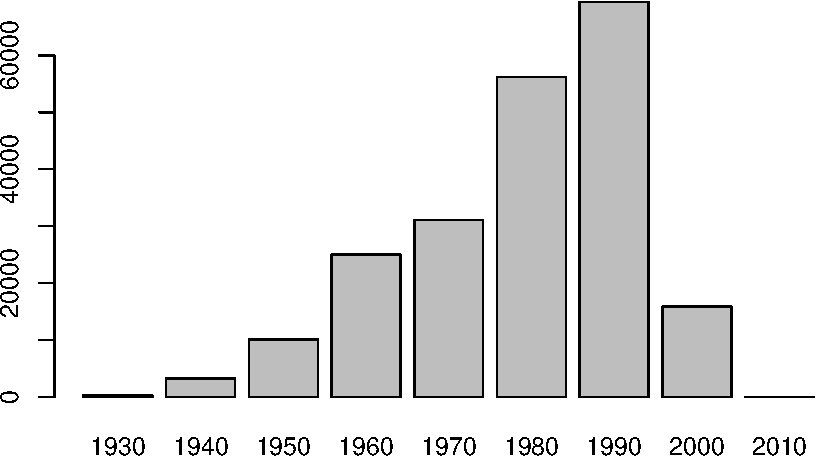
\includegraphics{R-data-wrangling_files/figure-latex/driver-birth-cohorts-1.pdf}
\caption{\label{fig:driver-birth-cohorts}Driver Birth Cohorts}
\end{figure}

Mutate can also be used in conjunction with logical conditions. For example, we could create a new column, where we assign everyone born after the year 2000 to a group ``millenial'' and overyone before to ``pre-millenial''.

In order to do this we take advantage of the \texttt{ifelse} function:

\texttt{ifelse(a\_logical\_condition,\ if\_true\_return\_this,\ if\_false\_return\_this)}

In conjunction with mutate, this works like this:

\begin{Shaded}
\begin{Highlighting}[]
\NormalTok{stops }\SpecialCharTok{\%\textgreater{}\%} 
  \FunctionTok{mutate}\NormalTok{(}\AttributeTok{cohort =} \FunctionTok{ifelse}\NormalTok{(}\FunctionTok{year}\NormalTok{(driver\_birthdate) }\SpecialCharTok{\textless{}} \DecValTok{2000}\NormalTok{, }\StringTok{"pre{-}millenial"}\NormalTok{, }\StringTok{"millenial"}\NormalTok{)) }\SpecialCharTok{\%\textgreater{}\%} 
  \FunctionTok{count}\NormalTok{(cohort)}
\end{Highlighting}
\end{Shaded}

\begin{verbatim}
#> # A tibble: 3 x 2
#>   cohort             n
#>   <chr>          <int>
#> 1 millenial         41
#> 2 pre-millenial 211061
#> 3 <NA>             109
\end{verbatim}

More advanced conditional recoding can be done with \href{https://dplyr.tidyverse.org/reference/case_when.html}{\texttt{case\_when()}}.

\begin{quote}
Challenge

Create a new data frame from the \texttt{stops} data that meets the following
criteria: contains only the \texttt{violation} column for female drivers of age 50 that were stopped on a Sunday. For this add a new column to your data frame called
\texttt{weekday\_of\_stop} containing the number of the weekday when the stop occurred. Use the \texttt{wday()} function from \texttt{lubridate} (Sunday = 1).

Think about how the commands should be ordered to produce this data frame!
\end{quote}

\hypertarget{what-is-split-apply-combine}{%
\section{What is split-apply-combine?}\label{what-is-split-apply-combine}}

Many data analysis tasks can be approached using the \emph{split-apply-combine}
paradigm: split the data into groups, apply some analysis to each group, and
then combine the results.

\begin{figure}
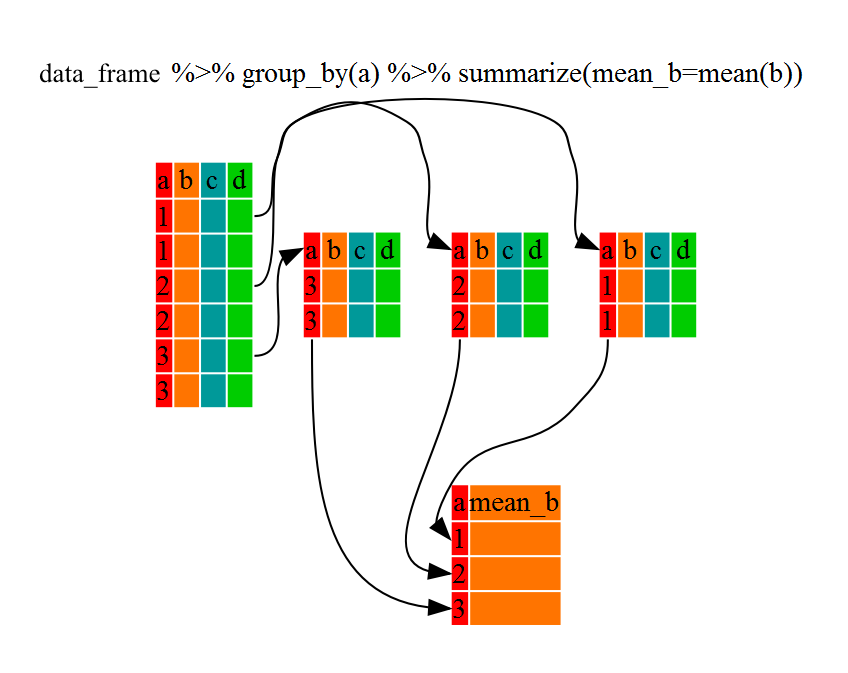
\includegraphics[width=\textwidth]{img/split-apply-combine} \caption{Split - Apply - Combine}\label{fig:split-apply-combine}
\end{figure}

\textbf{\texttt{dplyr}} makes this possible through the use of the \texttt{group\_by()} function.

\texttt{group\_by()} is often used together with \texttt{summarize()}, which collapses each
group into a single-row summary of that group. \texttt{group\_by()} takes as arguments
the column names that contain the \textbf{categorical} variables for which you want
to calculate the summary statistics. So to view the mean age for black and white drivers:

\begin{Shaded}
\begin{Highlighting}[]
\NormalTok{stops }\SpecialCharTok{\%\textgreater{}\%}
  \FunctionTok{group\_by}\NormalTok{(driver\_race) }\SpecialCharTok{\%\textgreater{}\%}
  \FunctionTok{summarize}\NormalTok{(}\AttributeTok{mean\_age =} \FunctionTok{mean}\NormalTok{(driver\_age, }\AttributeTok{na.rm=}\ConstantTok{TRUE}\NormalTok{))}
\end{Highlighting}
\end{Shaded}

\begin{verbatim}
#> `summarise()` ungrouping output (override with `.groups` argument)
\end{verbatim}

\begin{verbatim}
#> # A tibble: 3 x 2
#>   driver_race mean_age
#>   <chr>          <dbl>
#> 1 Black           34.2
#> 2 White           36.2
#> 3 <NA>            34.5
\end{verbatim}

You can also group by multiple columns:

\begin{Shaded}
\begin{Highlighting}[]
\NormalTok{stops }\SpecialCharTok{\%\textgreater{}\%} 
  \FunctionTok{group\_by}\NormalTok{(county\_name, driver\_race) }\SpecialCharTok{\%\textgreater{}\%}
  \FunctionTok{summarize}\NormalTok{(}\AttributeTok{mean\_age =} \FunctionTok{mean}\NormalTok{(driver\_age, }\AttributeTok{na.rm=}\ConstantTok{TRUE}\NormalTok{))}
\end{Highlighting}
\end{Shaded}

\begin{verbatim}
#> `summarise()` regrouping output by 'county_name' (override with `.groups` argument)
\end{verbatim}

\begin{verbatim}
#> # A tibble: 178 x 3
#> # Groups:   county_name [82]
#>    county_name driver_race mean_age
#>    <chr>       <chr>          <dbl>
#>  1 Adams       Black           36.2
#>  2 Adams       White           40.0
#>  3 Alcorn      Black           34.6
#>  4 Alcorn      White           33.6
#>  5 Amite       Black           37.5
#>  6 Amite       White           42.1
#>  7 Amite       <NA>            24  
#>  8 Attala      Black           36.4
#>  9 Attala      White           38.6
#> 10 Benton      Black           34.7
#> # ... with 168 more rows
\end{verbatim}

If we wanted to remove the line with \texttt{NA} we could insert a \texttt{filter()} in the chain:

\begin{Shaded}
\begin{Highlighting}[]
\NormalTok{stops }\SpecialCharTok{\%\textgreater{}\%}
  \FunctionTok{filter}\NormalTok{(}\SpecialCharTok{!}\FunctionTok{is.na}\NormalTok{(driver\_race)) }\SpecialCharTok{\%\textgreater{}\%} 
  \FunctionTok{group\_by}\NormalTok{(county\_name, driver\_race) }\SpecialCharTok{\%\textgreater{}\%}
  \FunctionTok{summarize}\NormalTok{(}\AttributeTok{mean\_age =} \FunctionTok{mean}\NormalTok{(driver\_age, }\AttributeTok{na.rm=}\ConstantTok{TRUE}\NormalTok{))}
\end{Highlighting}
\end{Shaded}

\begin{verbatim}
#> `summarise()` regrouping output by 'county_name' (override with `.groups` argument)
\end{verbatim}

\begin{verbatim}
#> # A tibble: 163 x 3
#> # Groups:   county_name [82]
#>    county_name driver_race mean_age
#>    <chr>       <chr>          <dbl>
#>  1 Adams       Black           36.2
#>  2 Adams       White           40.0
#>  3 Alcorn      Black           34.6
#>  4 Alcorn      White           33.6
#>  5 Amite       Black           37.5
#>  6 Amite       White           42.1
#>  7 Attala      Black           36.4
#>  8 Attala      White           38.6
#>  9 Benton      Black           34.7
#> 10 Benton      White           32.0
#> # ... with 153 more rows
\end{verbatim}

Recall that \texttt{is.na()} is a function that determines whether something is an \texttt{NA}. The \texttt{!} symbol negates the result, so we're asking for everything that is \emph{not} an \texttt{NA}.

Once the data are grouped, you can also summarize multiple variables at the same
time (and not necessarily on the same variable). For instance, we could add a
column indicating the minimum age in each group (i.e.~county):

\begin{Shaded}
\begin{Highlighting}[]
\NormalTok{stops }\SpecialCharTok{\%\textgreater{}\%}
  \FunctionTok{filter}\NormalTok{(}\SpecialCharTok{!}\FunctionTok{is.na}\NormalTok{(driver\_race)) }\SpecialCharTok{\%\textgreater{}\%} 
  \FunctionTok{group\_by}\NormalTok{(county\_name, driver\_race) }\SpecialCharTok{\%\textgreater{}\%}
  \FunctionTok{summarize}\NormalTok{(}\AttributeTok{mean\_age =} \FunctionTok{mean}\NormalTok{(driver\_age, }\AttributeTok{na.rm=}\ConstantTok{TRUE}\NormalTok{),}
            \AttributeTok{min\_age =} \FunctionTok{min}\NormalTok{(driver\_age, }\AttributeTok{na.rm=}\ConstantTok{TRUE}\NormalTok{))}
\end{Highlighting}
\end{Shaded}

\begin{verbatim}
#> `summarise()` regrouping output by 'county_name' (override with `.groups` argument)
\end{verbatim}

\begin{verbatim}
#> # A tibble: 163 x 4
#> # Groups:   county_name [82]
#>    county_name driver_race mean_age min_age
#>    <chr>       <chr>          <dbl>   <dbl>
#>  1 Adams       Black           36.2      16
#>  2 Adams       White           40.0      16
#>  3 Alcorn      Black           34.6      17
#>  4 Alcorn      White           33.6      15
#>  5 Amite       Black           37.5      17
#>  6 Amite       White           42.1      15
#>  7 Attala      Black           36.4       8
#>  8 Attala      White           38.6      15
#>  9 Benton      Black           34.7      18
#> 10 Benton      White           32.0      18
#> # ... with 153 more rows
\end{verbatim}

\hypertarget{tallying}{%
\section{Tallying}\label{tallying}}

When working with data, it is also common to want to know the number of
observations found for categorical variables. For this, \textbf{\texttt{dplyr}}
provides \texttt{count()}. For example, if we wanted to see how many traffic stops each officer recorded:

\begin{Shaded}
\begin{Highlighting}[]
\NormalTok{stops }\SpecialCharTok{\%\textgreater{}\%}
  \FunctionTok{count}\NormalTok{(officer\_id)}
\end{Highlighting}
\end{Shaded}

Bu default, count will name the column with the counts \texttt{n}. We can change this by explicitly providing a value for the \texttt{name} argument:

\begin{Shaded}
\begin{Highlighting}[]
\NormalTok{stops }\SpecialCharTok{\%\textgreater{}\%}
  \FunctionTok{count}\NormalTok{(officer\_id, }\AttributeTok{name =} \StringTok{"n\_stops"}\NormalTok{)}
\end{Highlighting}
\end{Shaded}

We can optionally sort the results in descending order by adding \texttt{sort=TRUE}:

\begin{Shaded}
\begin{Highlighting}[]
\NormalTok{stops }\SpecialCharTok{\%\textgreater{}\%}
  \FunctionTok{count}\NormalTok{(officer\_id, }\AttributeTok{name =} \StringTok{"n\_stops"}\NormalTok{, }\AttributeTok{sort =} \ConstantTok{TRUE}\NormalTok{)}
\end{Highlighting}
\end{Shaded}

\texttt{count()} calls \texttt{group\_by()} transparently before counting the total number of records for each category. Similarly, we can count subgroups within groups:

\begin{Shaded}
\begin{Highlighting}[]
\NormalTok{stops }\SpecialCharTok{\%\textgreater{}\%}
  \FunctionTok{count}\NormalTok{(officer\_id, violation, }\AttributeTok{name =} \StringTok{"n\_stops"}\NormalTok{)}
\end{Highlighting}
\end{Shaded}

Alternatives:

\begin{Shaded}
\begin{Highlighting}[]
\NormalTok{stops }\SpecialCharTok{\%\textgreater{}\%}
  \FunctionTok{group\_by}\NormalTok{(officer\_id) }\SpecialCharTok{\%\textgreater{}\%} 
  \FunctionTok{tally}\NormalTok{(}\AttributeTok{sort =} \ConstantTok{TRUE}\NormalTok{) }\CommentTok{\# tally() requires group\_by before counting}

\NormalTok{stops }\SpecialCharTok{\%\textgreater{}\%}
  \FunctionTok{group\_by}\NormalTok{(officer\_id) }\SpecialCharTok{\%\textgreater{}\%}
  \FunctionTok{summarize}\NormalTok{(}\AttributeTok{n =} \FunctionTok{n}\NormalTok{()) }\SpecialCharTok{\%\textgreater{}\%} \CommentTok{\# n() is useful when the count is needed within a calculation}
  \FunctionTok{arrange}\NormalTok{(}\FunctionTok{desc}\NormalTok{(n))}
\end{Highlighting}
\end{Shaded}

\begin{quote}
Challenge

Which 5 counties were the ones with the most stops in 2013?
Hint: use the year() function from lubridate.
\end{quote}

\hypertarget{joining-two-tables}{%
\section{Joining two tables}\label{joining-two-tables}}

It is not uncommon that we have our data spread out in different tables and need to bring those together for analysis. In this example we will combine the numbers of stops for black and white drivers per county together with the numbers of the black and white total population for these counties. The population data are the estimated values of the 5 year average from the 2011-2015 American Community Survey (ACS):

\begin{Shaded}
\begin{Highlighting}[]
\NormalTok{acs }\OtherTok{\textless{}{-}} \FunctionTok{read\_csv}\NormalTok{(}\StringTok{"data/MS\_acs2015\_bw.csv"}\NormalTok{)}
\end{Highlighting}
\end{Shaded}

\begin{verbatim}
#> Parsed with column specification:
#> cols(
#>   County = col_character(),
#>   FIPS = col_double(),
#>   black_pop = col_double(),
#>   white_pop = col_double(),
#>   bw_pop = col_double()
#> )
\end{verbatim}

\begin{Shaded}
\begin{Highlighting}[]
\NormalTok{acs}
\end{Highlighting}
\end{Shaded}

\begin{verbatim}
#> # A tibble: 82 x 5
#>    County      FIPS black_pop white_pop bw_pop
#>    <chr>      <dbl>     <dbl>     <dbl>  <dbl>
#>  1 Jones      28067     19711     47154  66865
#>  2 Lauderdale 28075     33893     43482  77375
#>  3 Pike       28113     21028     18282  39310
#>  4 Hancock    28045      4172     39686  43858
#>  5 Holmes     28051     15498      3105  18603
#>  6 Jackson    28059     30704    101686 132390
#>  7 Grenada    28043      9417     11991  21408
#>  8 Scott      28123     10562     16920  27482
#>  9 Wayne      28153      8015     12154  20169
#> 10 Bolivar    28011     21648     11197  32845
#> # ... with 72 more rows
\end{verbatim}

In a first step we count all the stops per county.

\begin{Shaded}
\begin{Highlighting}[]
\NormalTok{stops }\SpecialCharTok{\%\textgreater{}\%} 
  \FunctionTok{count}\NormalTok{(county\_name, }\AttributeTok{name =} \StringTok{"n\_stops"}\NormalTok{) }
\end{Highlighting}
\end{Shaded}

\begin{verbatim}
#> # A tibble: 82 x 2
#>    county_name n_stops
#>    <chr>         <int>
#>  1 Adams           942
#>  2 Alcorn         3345
#>  3 Amite          2921
#>  4 Attala         4203
#>  5 Benton          214
#>  6 Bolivar        4526
#>  7 Calhoun        1658
#>  8 Carroll        1788
#>  9 Chickasaw      3869
#> 10 Choctaw         613
#> # ... with 72 more rows
\end{verbatim}

We will then pipe this into our next operation where we bring the two tables together. We will use \texttt{left\_join}, which returns all rows from the left table, and all columns from the left and the right table. As ID, which uniquely identifies the corresponding records in each table we use the County names.

\begin{Shaded}
\begin{Highlighting}[]
\NormalTok{stops }\SpecialCharTok{\%\textgreater{}\%} 
  \FunctionTok{count}\NormalTok{(county\_name, }\AttributeTok{name =} \StringTok{"n\_stops"}\NormalTok{) }\SpecialCharTok{\%\textgreater{}\%} 
  \FunctionTok{left\_join}\NormalTok{(acs, }\AttributeTok{by =} \FunctionTok{c}\NormalTok{(}\StringTok{"county\_name"} \OtherTok{=} \StringTok{"County"}\NormalTok{)) }
\end{Highlighting}
\end{Shaded}

\begin{verbatim}
#> # A tibble: 82 x 6
#>    county_name n_stops  FIPS black_pop white_pop bw_pop
#>    <chr>         <int> <dbl>     <dbl>     <dbl>  <dbl>
#>  1 Adams           942 28001     17757     12856  30613
#>  2 Alcorn         3345 28003      4281     31563  35844
#>  3 Amite          2921 28005      5416      7395  12811
#>  4 Attala         4203 28007      8194     10649  18843
#>  5 Benton          214 28009      3078      5166   8244
#>  6 Bolivar        4526 28011     21648     11197  32845
#>  7 Calhoun        1658 28013      3991     10103  14094
#>  8 Carroll        1788 28015      3470      6702  10172
#>  9 Chickasaw      3869 28017      7549      9522  17071
#> 10 Choctaw         613 28019      2596      5661   8257
#> # ... with 72 more rows
\end{verbatim}

Now we can, for example calculate the stop rate, i.e.~the proportion of the population that gets stopped in each county.

\begin{quote}
Challenge

Which county has the highest and which one the lowest stop rate?
Use the snippet from above and pipe into the additional operations
to do this.
\end{quote}

\texttt{dplyr} join functions are generally equivalent to \texttt{merge} from the base command, but there are a few advantages:

\begin{itemize}
\tightlist
\item
  rows are kept in existing order
\item
  it runs faster
\item
  tells you what keys you're merging by (if you don't supply them)
\item
  also works with database tables.
\end{itemize}

\url{https://groups.google.com/d/msg/manipulatr/OuAPC4VyfIc/Qnt8mDfq0WwJ}

See \texttt{?dplyr::join} for all the possible joins.

\hypertarget{tidyr}{%
\chapter{\texorpdfstring{Data Manipulation using \textbf{\texttt{tidyr}}}{Data Manipulation using tidyr}}\label{tidyr}}

\begin{quote}
Learning Objectives

\begin{itemize}
\tightlist
\item
  Understand the concept of a wide and a long table format and for which purpose those formats are useful.
\item
  Understand what key-value pairs are.
\item
  Reshape a data frame from long to wide format and back with the \texttt{pivot\_wider} and \texttt{pivot\_longer} commands from the \textbf{\texttt{tidyr}} package.
\item
  Export a data frame to a .csv file.
\end{itemize}
\end{quote}

\begin{center}\rule{0.5\linewidth}{0.5pt}\end{center}

\texttt{dplyr} pairs nicely with \textbf{\texttt{tidyr}} which enables you to swiftly convert between different data formats for plotting and analysis.

The package \textbf{\texttt{tidyr}} addresses the common problem of wanting to reshape your data for plotting and use by different R functions. Sometimes we want data sets where we have one row per observation. Sometimes we want a data frame where each observation type has its own column, and rows are instead more aggregated groups - like surveys, where each column represents an answer. Moving back and forth between these formats is nontrivial, and \textbf{\texttt{tidyr}} gives you tools for this and more sophisticated data manipulation.

To learn more about \textbf{\texttt{tidyr}} after the workshop, you may want to check out this \href{https://github.com/rstudio/cheatsheets/raw/master/data-import.pdf}{cheatsheet about \textbf{\texttt{tidyr}}}.

\hypertarget{about-long-and-wide-table-format}{%
\section{About long and wide table format}\label{about-long-and-wide-table-format}}

The `long' format is where:

\begin{itemize}
\tightlist
\item
  each column is a variable
\item
  each row is an observation
\end{itemize}

In the `long' format, you usually have 1 column for the observed variable and
the other columns are ID variables.

For the `wide' format a row, for example could be a reserarch subject for which you have multiple observation variables containing the same type of data, for example responses to a set of survey questions, or repeated observations over time, or a mix of both. Here is an example:

\begin{table}[ht]
\centering
\begin{tabular}{rlrrr}
  \hline
 & subject\_ID & question\_1 & question\_2 & question\_3 \\ 
  \hline
1 & A & 4.00 & 3.00 & 4.00 \\ 
  2 & B & 4.00 & 1.00 & 5.00 \\ 
  3 & C & 2.00 & 5.00 & 2.00 \\ 
   \hline
\end{tabular}
\end{table}

You may find data input may be simpler or some other
applications may prefer the `wide' format. However, many of \texttt{R}`s functions have
been designed assuming you have 'long' format data. This tutorial will help you
efficiently transform your data regardless of original format.

\begin{figure}
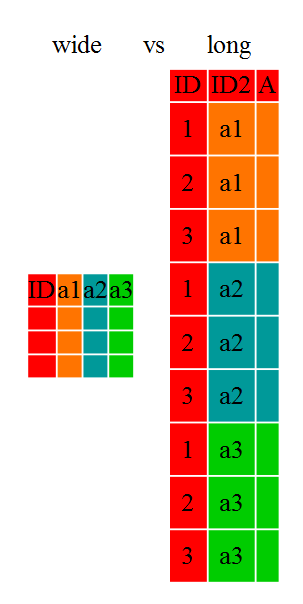
\includegraphics[width=0.3\linewidth]{img/wide-vs-long} \caption{Wide vs. Long Table Format}\label{fig:wide-vs-long}
\end{figure}

The choice of data format affects readability. For humans, the wide format is often more intuitive, since we can often see more of the data on the screen due to its shape. However, the long format is more machine readable and is closer to the formatting of databases. The \texttt{ID} variables in our dataframes are similar to the fields in a database and observed variables are like the database values.

\begin{quote}
Challenge 1

Is stops in a long or wide format?
\end{quote}

\hypertarget{long-to-wide-with-pivot_wider}{%
\section{\texorpdfstring{Long to Wide with \texttt{pivot\_wider}}{Long to Wide with pivot\_wider}}\label{long-to-wide-with-pivot_wider}}

Now let's see this in action. First, using \textbf{\texttt{dplyr}}, let's create a data frame with the counts of different violations for each county:

\begin{Shaded}
\begin{Highlighting}[]
\NormalTok{violations }\OtherTok{\textless{}{-}}\NormalTok{ stops }\SpecialCharTok{\%\textgreater{}\%}
  \FunctionTok{count}\NormalTok{(county\_name, violation)}

\NormalTok{violations}
\end{Highlighting}
\end{Shaded}

\begin{verbatim}
#>         county_name                violation    n
#> 1             Adams        Breaks-Lights-etc    7
#> 2             Adams         Careless driving   48
#> 3             Adams License-Permit-Insurance  118
#> 4             Adams         Other or unknown   35
#> 5             Adams                Seat belt  229
#> 6             Adams                 Speeding  505
#> 7            Alcorn        Breaks-Lights-etc   62
#> 8            Alcorn         Careless driving  100
#> 9            Alcorn License-Permit-Insurance  737
#> 10           Alcorn         Other or unknown  418
#> 11           Alcorn                Seat belt  629
#> 12           Alcorn                 Speeding 1399
#> 13            Amite        Breaks-Lights-etc   47
#> 14            Amite         Careless driving   86
#> 15            Amite License-Permit-Insurance  370
#> 16            Amite         Other or unknown  143
#> 17            Amite                Seat belt  336
#> 18            Amite                 Speeding 1939
#> 19           Attala        Breaks-Lights-etc   99
#> 20           Attala         Careless driving  113
#> 21           Attala License-Permit-Insurance  526
#> 22           Attala         Other or unknown  155
#> 23           Attala                Seat belt  748
#> 24           Attala                 Speeding 2562
#> 25           Benton        Breaks-Lights-etc    3
#> 26           Benton         Careless driving    9
#> 27           Benton License-Permit-Insurance   73
#> 28           Benton         Other or unknown   26
#> 29           Benton                Seat belt   29
#> 30           Benton                 Speeding   74
#> 31          Bolivar        Breaks-Lights-etc   57
#> 32          Bolivar         Careless driving  139
#> 33          Bolivar License-Permit-Insurance 1034
#> 34          Bolivar         Other or unknown  254
#> 35          Bolivar                Seat belt  729
#> 36          Bolivar                 Speeding 2313
#> 37          Calhoun        Breaks-Lights-etc   26
#> 38          Calhoun         Careless driving   38
#> 39          Calhoun License-Permit-Insurance  383
#> 40          Calhoun         Other or unknown  102
#> 41          Calhoun                Seat belt  150
#> 42          Calhoun                 Speeding  959
#> 43          Carroll        Breaks-Lights-etc   26
#> 44          Carroll         Careless driving   40
#> 45          Carroll License-Permit-Insurance  323
#> 46          Carroll         Other or unknown  103
#> 47          Carroll                Seat belt  158
#> 48          Carroll                 Speeding 1138
#> 49        Chickasaw        Breaks-Lights-etc   42
#> 50        Chickasaw         Careless driving   53
#> 51        Chickasaw License-Permit-Insurance 1378
#> 52        Chickasaw         Other or unknown  232
#> 53        Chickasaw                Seat belt  442
#> 54        Chickasaw                 Speeding 1722
#> 55          Choctaw        Breaks-Lights-etc    8
#> 56          Choctaw         Careless driving    6
#> 57          Choctaw License-Permit-Insurance   73
#> 58          Choctaw         Other or unknown   24
#> 59          Choctaw                Seat belt   18
#> 60          Choctaw                 Speeding  484
#> 61        Claiborne        Breaks-Lights-etc   25
#> 62        Claiborne         Careless driving   39
#> 63        Claiborne License-Permit-Insurance  102
#> 64        Claiborne         Other or unknown  162
#> 65        Claiborne                Seat belt  177
#> 66        Claiborne                 Speeding  882
#> 67           Clarke        Breaks-Lights-etc    8
#> 68           Clarke         Careless driving   15
#> 69           Clarke License-Permit-Insurance  169
#> 70           Clarke         Other or unknown   66
#> 71           Clarke                Seat belt   33
#> 72           Clarke                 Speeding  294
#> 73             Clay        Breaks-Lights-etc   39
#> 74             Clay         Careless driving   48
#> 75             Clay License-Permit-Insurance  424
#> 76             Clay         Other or unknown   86
#> 77             Clay                Seat belt  105
#> 78             Clay                 Speeding  279
#> 79          Coahoma        Breaks-Lights-etc   17
#> 80          Coahoma         Careless driving   55
#> 81          Coahoma License-Permit-Insurance  410
#> 82          Coahoma         Other or unknown  440
#> 83          Coahoma                Seat belt  401
#> 84          Coahoma                 Speeding 1268
#> 85           Copiah        Breaks-Lights-etc  140
#> 86           Copiah         Careless driving  215
#> 87           Copiah License-Permit-Insurance  993
#> 88           Copiah         Other or unknown  337
#> 89           Copiah                Seat belt  850
#> 90           Copiah                 Speeding 3551
#> 91        Covington        Breaks-Lights-etc   11
#> 92        Covington         Careless driving   66
#> 93        Covington License-Permit-Insurance  714
#> 94        Covington         Other or unknown  135
#> 95        Covington                Seat belt   98
#> 96        Covington                 Speeding  874
#> 97           DeSoto        Breaks-Lights-etc   40
#> 98           DeSoto         Careless driving   61
#> 99           DeSoto License-Permit-Insurance  187
#> 100          DeSoto         Other or unknown  123
#> 101          DeSoto                Seat belt  145
#> 102          DeSoto                 Speeding  647
#> 103         Forrest        Breaks-Lights-etc   57
#> 104         Forrest         Careless driving  264
#> 105         Forrest License-Permit-Insurance  969
#> 106         Forrest         Other or unknown  457
#> 107         Forrest                Seat belt  261
#> 108         Forrest                 Speeding 2427
#> 109        Franklin        Breaks-Lights-etc   26
#> 110        Franklin         Careless driving   61
#> 111        Franklin License-Permit-Insurance  408
#> 112        Franklin         Other or unknown  155
#> 113        Franklin                Seat belt  339
#> 114        Franklin                 Speeding 1518
#> 115          George        Breaks-Lights-etc   33
#> 116          George         Careless driving   88
#> 117          George License-Permit-Insurance  820
#> 118          George         Other or unknown  360
#> 119          George                Seat belt  355
#> 120          George                 Speeding 3122
#> 121          Greene        Breaks-Lights-etc    5
#> 122          Greene         Careless driving   35
#> 123          Greene License-Permit-Insurance  148
#> 124          Greene         Other or unknown   57
#> 125          Greene                Seat belt   21
#> 126          Greene                 Speeding  787
#> 127         Grenada        Breaks-Lights-etc   33
#> 128         Grenada         Careless driving   45
#> 129         Grenada License-Permit-Insurance  506
#> 130         Grenada         Other or unknown  196
#> 131         Grenada                Seat belt  180
#> 132         Grenada                 Speeding 1684
#> 133         Hancock        Breaks-Lights-etc  213
#> 134         Hancock         Careless driving   90
#> 135         Hancock License-Permit-Insurance  344
#> 136         Hancock         Other or unknown  145
#> 137         Hancock                Seat belt  563
#> 138         Hancock                 Speeding 2435
#> 139        Harrison        Breaks-Lights-etc  212
#> 140        Harrison         Careless driving  312
#> 141        Harrison License-Permit-Insurance 1273
#> 142        Harrison         Other or unknown  443
#> 143        Harrison                Seat belt  306
#> 144        Harrison                 Speeding 3550
#> 145           Hinds        Breaks-Lights-etc  136
#> 146           Hinds         Careless driving  264
#> 147           Hinds License-Permit-Insurance  648
#> 148           Hinds         Other or unknown  695
#> 149           Hinds                Seat belt  609
#> 150           Hinds                 Speeding 2641
#> 151          Holmes        Breaks-Lights-etc   23
#> 152          Holmes         Careless driving   91
#> 153          Holmes License-Permit-Insurance  375
#> 154          Holmes         Other or unknown  228
#> 155          Holmes                Seat belt  350
#> 156          Holmes                 Speeding 3249
#> 157       Humphreys        Breaks-Lights-etc    3
#> 158       Humphreys         Careless driving    8
#> 159       Humphreys License-Permit-Insurance  199
#> 160       Humphreys         Other or unknown   35
#> 161       Humphreys                Seat belt   37
#> 162       Humphreys                 Speeding 1836
#> 163       Issaquena        Breaks-Lights-etc    9
#> 164       Issaquena         Careless driving    4
#> 165       Issaquena License-Permit-Insurance   23
#> 166       Issaquena         Other or unknown  261
#> 167       Issaquena                Seat belt  230
#> 168       Issaquena                 Speeding  610
#> 169        Itawamba        Breaks-Lights-etc   66
#> 170        Itawamba         Careless driving  128
#> 171        Itawamba License-Permit-Insurance  640
#> 172        Itawamba         Other or unknown  160
#> 173        Itawamba                Seat belt  740
#> 174        Itawamba                 Speeding  747
#> 175         Jackson        Breaks-Lights-etc  111
#> 176         Jackson         Careless driving  532
#> 177         Jackson License-Permit-Insurance  662
#> 178         Jackson         Other or unknown  490
#> 179         Jackson                Seat belt  669
#> 180         Jackson                 Speeding 4295
#> 181          Jasper        Breaks-Lights-etc   13
#> 182          Jasper         Careless driving   46
#> 183          Jasper License-Permit-Insurance  368
#> 184          Jasper         Other or unknown  109
#> 185          Jasper                Seat belt   81
#> 186          Jasper                 Speeding 1391
#> 187       Jefferson        Breaks-Lights-etc  173
#> 188       Jefferson         Careless driving   98
#> 189       Jefferson License-Permit-Insurance  670
#> 190       Jefferson         Other or unknown  315
#> 191       Jefferson                Seat belt  420
#> 192       Jefferson                 Speeding 2536
#> 193 Jefferson Davis        Breaks-Lights-etc    4
#> 194 Jefferson Davis         Careless driving   46
#> 195 Jefferson Davis License-Permit-Insurance  225
#> 196 Jefferson Davis         Other or unknown   47
#> 197 Jefferson Davis                Seat belt   29
#> 198 Jefferson Davis                 Speeding  607
#> 199           Jones        Breaks-Lights-etc   22
#> 200           Jones         Careless driving  162
#> 201           Jones License-Permit-Insurance  674
#> 202           Jones         Other or unknown  257
#> 203           Jones                Seat belt  300
#> 204           Jones                 Speeding 2418
#> 205          Kemper        Breaks-Lights-etc   24
#> 206          Kemper         Careless driving   16
#> 207          Kemper License-Permit-Insurance  129
#> 208          Kemper         Other or unknown  105
#> 209          Kemper                Seat belt  109
#> 210          Kemper                 Speeding 2117
#> 211       Lafayette        Breaks-Lights-etc   12
#> 212       Lafayette         Careless driving   57
#> 213       Lafayette License-Permit-Insurance  140
#> 214       Lafayette         Other or unknown   89
#> 215       Lafayette                Seat belt  261
#> 216       Lafayette                 Speeding  610
#> 217           Lamar        Breaks-Lights-etc   31
#> 218           Lamar         Careless driving   99
#> 219           Lamar License-Permit-Insurance  506
#> 220           Lamar         Other or unknown  264
#> 221           Lamar                Seat belt  150
#> 222           Lamar                 Speeding 2315
#> 223      Lauderdale        Breaks-Lights-etc   50
#> 224      Lauderdale         Careless driving  354
#> 225      Lauderdale License-Permit-Insurance  949
#> 226      Lauderdale         Other or unknown  535
#> 227      Lauderdale                Seat belt  403
#> 228      Lauderdale                 Speeding 6504
#> 229        Lawrence        Breaks-Lights-etc    9
#> 230        Lawrence         Careless driving   13
#> 231        Lawrence License-Permit-Insurance  108
#> 232        Lawrence         Other or unknown   39
#> 233        Lawrence                Seat belt   52
#> 234        Lawrence                 Speeding  347
#> 235           Leake        Breaks-Lights-etc   16
#> 236           Leake         Careless driving   57
#> 237           Leake License-Permit-Insurance  322
#> 238           Leake         Other or unknown   81
#> 239           Leake                Seat belt  131
#> 240           Leake                 Speeding 2390
#> 241             Lee        Breaks-Lights-etc   97
#> 242             Lee         Careless driving  182
#> 243             Lee License-Permit-Insurance  833
#> 244             Lee         Other or unknown  202
#> 245             Lee                Seat belt  937
#> 246             Lee                 Speeding 2709
#> 247         Leflore        Breaks-Lights-etc   45
#> 248         Leflore         Careless driving   59
#> 249         Leflore License-Permit-Insurance  611
#> 250         Leflore         Other or unknown  153
#> 251         Leflore                Seat belt  195
#> 252         Leflore                 Speeding  611
#> 253         Lincoln        Breaks-Lights-etc   22
#> 254         Lincoln         Careless driving   83
#> 255         Lincoln License-Permit-Insurance  264
#> 256         Lincoln         Other or unknown  100
#> 257         Lincoln                Seat belt  408
#> 258         Lincoln                 Speeding 2951
#> 259         Lowndes        Breaks-Lights-etc   28
#> 260         Lowndes         Careless driving  130
#> 261         Lowndes License-Permit-Insurance  456
#> 262         Lowndes         Other or unknown   71
#> 263         Lowndes                Seat belt  235
#> 264         Lowndes                 Speeding 2290
#> 265         Madison        Breaks-Lights-etc   50
#> 266         Madison         Careless driving   73
#> 267         Madison License-Permit-Insurance  270
#> 268         Madison         Other or unknown   79
#> 269         Madison                Seat belt   86
#> 270         Madison                 Speeding 1451
#> 271          Marion        Breaks-Lights-etc    7
#> 272          Marion         Careless driving   13
#> 273          Marion License-Permit-Insurance  103
#> 274          Marion         Other or unknown   22
#> 275          Marion                Seat belt   28
#> 276          Marion                 Speeding   66
#> 277        Marshall        Breaks-Lights-etc   14
#> 278        Marshall         Careless driving    8
#> 279        Marshall License-Permit-Insurance   40
#> 280        Marshall         Other or unknown   38
#> 281        Marshall                Seat belt   40
#> 282        Marshall                 Speeding   80
#> 283          Monroe        Breaks-Lights-etc  190
#> 284          Monroe         Careless driving  200
#> 285          Monroe License-Permit-Insurance 2889
#> 286          Monroe         Other or unknown  549
#> 287          Monroe                Seat belt 1300
#> 288          Monroe                 Speeding 5341
#> 289      Montgomery        Breaks-Lights-etc   79
#> 290      Montgomery         Careless driving   69
#> 291      Montgomery License-Permit-Insurance  573
#> 292      Montgomery         Other or unknown  150
#> 293      Montgomery                Seat belt  187
#> 294      Montgomery                 Speeding 2325
#> 295         Neshoba        Breaks-Lights-etc    1
#> 296         Neshoba         Careless driving    3
#> 297         Neshoba License-Permit-Insurance   19
#> 298         Neshoba         Other or unknown   20
#> 299         Neshoba                Seat belt    4
#> 300         Neshoba                 Speeding   30
#> 301          Newton        Breaks-Lights-etc   28
#> 302          Newton         Careless driving   50
#> 303          Newton License-Permit-Insurance  334
#> 304          Newton         Other or unknown  254
#> 305          Newton                Seat belt  308
#> 306          Newton                 Speeding 1511
#> 307         Noxubee        Breaks-Lights-etc    1
#> 308         Noxubee         Careless driving    1
#> 309         Noxubee License-Permit-Insurance   10
#> 310         Noxubee         Other or unknown    5
#> 311         Noxubee                Seat belt    2
#> 312         Noxubee                 Speeding   11
#> 313       Oktibbeha        Breaks-Lights-etc   13
#> 314       Oktibbeha         Careless driving   69
#> 315       Oktibbeha License-Permit-Insurance  818
#> 316       Oktibbeha         Other or unknown  151
#> 317       Oktibbeha                Seat belt  215
#> 318       Oktibbeha                 Speeding 2734
#> 319          Panola        Breaks-Lights-etc   15
#> 320          Panola         Careless driving  100
#> 321          Panola License-Permit-Insurance  206
#> 322          Panola         Other or unknown   77
#> 323          Panola                Seat belt  387
#> 324          Panola                 Speeding  969
#> 325     Pearl River        Breaks-Lights-etc   16
#> 326     Pearl River         Careless driving   14
#> 327     Pearl River License-Permit-Insurance  301
#> 328     Pearl River         Other or unknown  166
#> 329     Pearl River                Seat belt   32
#> 330     Pearl River                 Speeding  316
#> 331           Perry        Breaks-Lights-etc    6
#> 332           Perry         Careless driving    5
#> 333           Perry License-Permit-Insurance   65
#> 334           Perry         Other or unknown   41
#> 335           Perry                Seat belt   26
#> 336           Perry                 Speeding  642
#> 337            Pike        Breaks-Lights-etc   47
#> 338            Pike         Careless driving  163
#> 339            Pike License-Permit-Insurance  752
#> 340            Pike         Other or unknown  329
#> 341            Pike                Seat belt  490
#> 342            Pike                 Speeding 2387
#> 343        Pontotoc        Breaks-Lights-etc   16
#> 344        Pontotoc         Careless driving   79
#> 345        Pontotoc License-Permit-Insurance  300
#> 346        Pontotoc         Other or unknown   89
#> 347        Pontotoc                Seat belt  111
#> 348        Pontotoc                 Speeding 1057
#> 349        Prentiss        Breaks-Lights-etc   23
#> 350        Prentiss         Careless driving   65
#> 351        Prentiss License-Permit-Insurance  296
#> 352        Prentiss         Other or unknown  137
#> 353        Prentiss                Seat belt  377
#> 354        Prentiss                 Speeding 1143
#> 355         Quitman        Breaks-Lights-etc   14
#> 356         Quitman         Careless driving   47
#> 357         Quitman License-Permit-Insurance  166
#> 358         Quitman         Other or unknown   87
#> 359         Quitman                Seat belt  223
#> 360         Quitman                 Speeding  978
#> 361          Rankin        Breaks-Lights-etc    5
#> 362          Rankin         Careless driving   25
#> 363          Rankin License-Permit-Insurance  100
#> 364          Rankin         Other or unknown   41
#> 365          Rankin                Seat belt   29
#> 366          Rankin                 Speeding  156
#> 367           Scott        Breaks-Lights-etc   41
#> 368           Scott         Careless driving  208
#> 369           Scott License-Permit-Insurance 1237
#> 370           Scott         Other or unknown  234
#> 371           Scott                Seat belt  649
#> 372           Scott                 Speeding 2556
#> 373         Sharkey        Breaks-Lights-etc   11
#> 374         Sharkey         Careless driving   12
#> 375         Sharkey License-Permit-Insurance   43
#> 376         Sharkey         Other or unknown  448
#> 377         Sharkey                Seat belt  328
#> 378         Sharkey                 Speeding  930
#> 379         Simpson        Breaks-Lights-etc   78
#> 380         Simpson         Careless driving   96
#> 381         Simpson License-Permit-Insurance  760
#> 382         Simpson         Other or unknown  219
#> 383         Simpson                Seat belt  293
#> 384         Simpson                 Speeding 2035
#> 385           Smith        Breaks-Lights-etc    2
#> 386           Smith         Careless driving    9
#> 387           Smith License-Permit-Insurance   20
#> 388           Smith         Other or unknown   18
#> 389           Smith                Seat belt    5
#> 390           Smith                 Speeding  206
#> 391           Stone        Breaks-Lights-etc   35
#> 392           Stone         Careless driving   80
#> 393           Stone License-Permit-Insurance  298
#> 394           Stone         Other or unknown  180
#> 395           Stone                Seat belt  180
#> 396           Stone                 Speeding 2135
#> 397       Sunflower        Breaks-Lights-etc   28
#> 398       Sunflower         Careless driving  119
#> 399       Sunflower License-Permit-Insurance 1084
#> 400       Sunflower         Other or unknown  144
#> 401       Sunflower                Seat belt  518
#> 402       Sunflower                 Speeding 2029
#> 403    Tallahatchie        Breaks-Lights-etc    8
#> 404    Tallahatchie         Careless driving    6
#> 405    Tallahatchie License-Permit-Insurance   34
#> 406    Tallahatchie         Other or unknown   29
#> 407    Tallahatchie                Seat belt   60
#> 408    Tallahatchie                 Speeding  256
#> 409            Tate        Breaks-Lights-etc   50
#> 410            Tate         Careless driving   70
#> 411            Tate License-Permit-Insurance  335
#> 412            Tate         Other or unknown  126
#> 413            Tate                Seat belt  316
#> 414            Tate                 Speeding 1080
#> 415          Tippah        Breaks-Lights-etc   12
#> 416          Tippah         Careless driving   58
#> 417          Tippah License-Permit-Insurance  449
#> 418          Tippah         Other or unknown  115
#> 419          Tippah                Seat belt  357
#> 420          Tippah                 Speeding  488
#> 421      Tishomingo        Breaks-Lights-etc   31
#> 422      Tishomingo         Careless driving   41
#> 423      Tishomingo License-Permit-Insurance  278
#> 424      Tishomingo         Other or unknown  163
#> 425      Tishomingo                Seat belt  433
#> 426      Tishomingo                 Speeding  746
#> 427          Tunica License-Permit-Insurance    2
#> 428          Tunica         Other or unknown    1
#> 429          Tunica                 Speeding    1
#> 430           Union        Breaks-Lights-etc    4
#> 431           Union         Careless driving   69
#> 432           Union License-Permit-Insurance  360
#> 433           Union         Other or unknown  174
#> 434           Union                Seat belt  442
#> 435           Union                 Speeding 1413
#> 436        Walthall        Breaks-Lights-etc   10
#> 437        Walthall         Careless driving   34
#> 438        Walthall License-Permit-Insurance  266
#> 439        Walthall         Other or unknown  175
#> 440        Walthall                Seat belt  156
#> 441        Walthall                 Speeding 1181
#> 442          Warren        Breaks-Lights-etc   36
#> 443          Warren         Careless driving   29
#> 444          Warren License-Permit-Insurance  183
#> 445          Warren         Other or unknown  360
#> 446          Warren                Seat belt  551
#> 447          Warren                 Speeding 1570
#> 448      Washington        Breaks-Lights-etc   31
#> 449      Washington         Careless driving   49
#> 450      Washington License-Permit-Insurance  227
#> 451      Washington         Other or unknown  106
#> 452      Washington                Seat belt  557
#> 453      Washington                 Speeding 1775
#> 454           Wayne        Breaks-Lights-etc    8
#> 455           Wayne         Careless driving  159
#> 456           Wayne License-Permit-Insurance  415
#> 457           Wayne         Other or unknown  163
#> 458           Wayne                Seat belt  461
#> 459           Wayne                 Speeding 3041
#> 460         Webster        Breaks-Lights-etc    1
#> 461         Webster License-Permit-Insurance   14
#> 462         Webster         Other or unknown    1
#> 463         Webster                Seat belt   10
#> 464         Webster                 Speeding  130
#> 465       Wilkinson        Breaks-Lights-etc    1
#> 466       Wilkinson License-Permit-Insurance   16
#> 467       Wilkinson         Other or unknown    6
#> 468       Wilkinson                Seat belt    5
#> 469       Wilkinson                 Speeding   15
#> 470         Winston        Breaks-Lights-etc   27
#> 471         Winston         Careless driving   85
#> 472         Winston License-Permit-Insurance  696
#> 473         Winston         Other or unknown  290
#> 474         Winston                Seat belt  294
#> 475         Winston                 Speeding 2930
#> 476       Yalobusha        Breaks-Lights-etc    3
#> 477       Yalobusha         Careless driving   13
#> 478       Yalobusha License-Permit-Insurance   48
#> 479       Yalobusha         Other or unknown   25
#> 480       Yalobusha                Seat belt  125
#> 481       Yalobusha                 Speeding  108
#> 482           Yazoo        Breaks-Lights-etc   28
#> 483           Yazoo         Careless driving   86
#> 484           Yazoo License-Permit-Insurance  239
#> 485           Yazoo         Other or unknown  105
#> 486           Yazoo                Seat belt  202
#> 487           Yazoo                 Speeding 2868
\end{verbatim}

Now, to make this long data wide, we use \texttt{pivot\_wider} from \texttt{tidyr} to turn the driver gender into columns. In addition to our data table we provide \texttt{pivot\_wider} with two arguments: \texttt{names\_from} describes which column to use for name of the output column, and \texttt{values\_from} tells it from column to get the cell values. We'll use a pipe so we can ignore the data argument.

\begin{Shaded}
\begin{Highlighting}[]
\NormalTok{violations\_wide }\OtherTok{\textless{}{-}}\NormalTok{ violations }\SpecialCharTok{\%\textgreater{}\%}
  \FunctionTok{pivot\_wider}\NormalTok{(}\AttributeTok{names\_from =}\NormalTok{ violation, }
              \AttributeTok{values\_from =}\NormalTok{ n) }

\NormalTok{violations\_wide}
\end{Highlighting}
\end{Shaded}

\begin{verbatim}
#> # A tibble: 82 x 7
#>    county_name `Breaks-Lights-~ `Careless drivi~ `License-Permit~
#>    <chr>                  <int>            <int>            <int>
#>  1 Adams                      7               48              118
#>  2 Alcorn                    62              100              737
#>  3 Amite                     47               86              370
#>  4 Attala                    99              113              526
#>  5 Benton                     3                9               73
#>  6 Bolivar                   57              139             1034
#>  7 Calhoun                   26               38              383
#>  8 Carroll                   26               40              323
#>  9 Chickasaw                 42               53             1378
#> 10 Choctaw                    8                6               73
#> # ... with 72 more rows, and 3 more variables: `Other or unknown` <int>, `Seat
#> #   belt` <int>, Speeding <int>
\end{verbatim}

\hypertarget{wide-to-long-with-pivot_longer}{%
\section{\texorpdfstring{Wide to long with \texttt{pivot\_longer}}{Wide to long with pivot\_longer}}\label{wide-to-long-with-pivot_longer}}

What if we had the opposite problem, and wanted to go from a wide to long
format? For that, we use \texttt{pivot\_longer}, which will increase the number of rows and decrease the number of columns. We provide the functino with thee arguments: \texttt{cols} which are the columns we want to pivot into the long format, \texttt{names\_to}, which is a string specifying the name of the column to create from the data stored in the column names, and \texttt{values\_to}, which is also a string, specifying the name of the column to create from the data stored in cell values.
So, to go backwards from \texttt{violations\_wide}, and exclude \texttt{county\_name} from the long format, we would do the following:

\begin{Shaded}
\begin{Highlighting}[]
\NormalTok{violations\_long }\OtherTok{\textless{}{-}}\NormalTok{ violations\_wide }\SpecialCharTok{\%\textgreater{}\%}
  \FunctionTok{pivot\_longer}\NormalTok{(}\AttributeTok{cols =} \SpecialCharTok{{-}}\NormalTok{county\_name,        }\CommentTok{\# exclude column with county name}
               \AttributeTok{names\_to =} \StringTok{"violation"}\NormalTok{,     }\CommentTok{\# name is a string!}
               \AttributeTok{values\_to =} \StringTok{"n"}\NormalTok{)            }\CommentTok{\# also a string}

\NormalTok{violations\_long}
\end{Highlighting}
\end{Shaded}

\begin{verbatim}
#> # A tibble: 492 x 3
#>    county_name violation                    n
#>    <chr>       <chr>                    <int>
#>  1 Adams       Breaks-Lights-etc            7
#>  2 Adams       Careless driving            48
#>  3 Adams       License-Permit-Insurance   118
#>  4 Adams       Other or unknown            35
#>  5 Adams       Seat belt                  229
#>  6 Adams       Speeding                   505
#>  7 Alcorn      Breaks-Lights-etc           62
#>  8 Alcorn      Careless driving           100
#>  9 Alcorn      License-Permit-Insurance   737
#> 10 Alcorn      Other or unknown           418
#> # ... with 482 more rows
\end{verbatim}

We could also have used a specification for what columns to include. This can be
useful if you have a large number of identifying columns, and it's easier to
specify what to gather than what to leave alone. And if the columns are adjacent to each other, we don't even need to list them all out -- we can use the \texttt{:} operator!

\begin{Shaded}
\begin{Highlighting}[]
\NormalTok{violations\_wide }\SpecialCharTok{\%\textgreater{}\%}
  \FunctionTok{pivot\_longer}\NormalTok{(}\AttributeTok{cols =} \StringTok{\textasciigrave{}}\AttributeTok{Breaks{-}Lights{-}etc}\StringTok{\textasciigrave{}}\SpecialCharTok{:}\NormalTok{Speeding,      }\CommentTok{\# this also works}
               \AttributeTok{names\_to =} \StringTok{"violation"}\NormalTok{, }
               \AttributeTok{values\_to =} \StringTok{"n"}\NormalTok{)}
\end{Highlighting}
\end{Shaded}

\begin{verbatim}
#> # A tibble: 492 x 3
#>    county_name violation                    n
#>    <chr>       <chr>                    <int>
#>  1 Adams       Breaks-Lights-etc            7
#>  2 Adams       Careless driving            48
#>  3 Adams       License-Permit-Insurance   118
#>  4 Adams       Other or unknown            35
#>  5 Adams       Seat belt                  229
#>  6 Adams       Speeding                   505
#>  7 Alcorn      Breaks-Lights-etc           62
#>  8 Alcorn      Careless driving           100
#>  9 Alcorn      License-Permit-Insurance   737
#> 10 Alcorn      Other or unknown           418
#> # ... with 482 more rows
\end{verbatim}

There are many powerful operations you can do with the \texttt{pivot\_*} functions. To learn more review the vignette:

\begin{Shaded}
\begin{Highlighting}[]
\FunctionTok{vignette}\NormalTok{(}\StringTok{"pivot"}\NormalTok{)}
\end{Highlighting}
\end{Shaded}

\begin{quote}
Challenge

1.From the stops dataframe create a wide data frame \texttt{tr\_wide} with
``year'' as columns, each row is a different violation,
and the values are the
number of traffic stops per each violation, roughly like this:

\texttt{violation\ \ \ \ \ \ \textbar{}\ 2013\ \textbar{}\ 2014\ \textbar{}\ 2015\ ...}
\texttt{Break-Lights\ \ \ \textbar{}\ \ \ 65\ \textbar{}\ \ \ \ 54\textbar{}\ \ \ 67\ ...}
\texttt{Speeding\ \ \ \ \ \ \ \textbar{}\ \ 713\ \textbar{}\ \ \ 948\textbar{}\ \ 978\ ...}
\texttt{...}

Use \texttt{year()} from the lubridate package. Hint: You will need to summarize
and count the traffic stops before reshaping the table.
\end{quote}

\begin{quote}
\begin{enumerate}
\def\labelenumi{\arabic{enumi}.}
\setcounter{enumi}{1}
\tightlist
\item
  Now take the data frame, and make it long again, so each row is a
  unique violation - year combination, like this:
\end{enumerate}

\texttt{violation\ \ \textbar{}\ year\ \textbar{}\ n\ of\ stops}
\texttt{Speeding\ \ \ \textbar{}\ 2013\ \textbar{}\ 65}
\texttt{Speeding\ \ \ \textbar{}\ 2014\ \textbar{}\ 54}
\texttt{...\ etc}
\end{quote}

\hypertarget{exporting-data}{%
\section{Exporting data}\label{exporting-data}}

Similar to the \texttt{read\_csv()} function used for reading CSV files into R, there is a \texttt{write\_csv()} function that generates CSV files from data frames.

Before using \texttt{write\_csv()}, we are going to create a new folder, \texttt{data\_output},
in our working directory that will store this generated dataset. We don't want
to write generated datasets in the same directory as our raw data. It's good
practice to keep them separate. The \texttt{data} folder should only contain the raw,
unaltered data, and should be left alone to make sure we don't delete or modify
it. In contrast, our script will generate the contents of the \texttt{data\_output}
directory, so even if the files it contains are deleted, we can always
re-generate them.

We can now save the table generated above in our \texttt{data\_output}
folder:

\begin{Shaded}
\begin{Highlighting}[]
\FunctionTok{write\_csv}\NormalTok{(violation\_wide, }\StringTok{"data\_output/county\_violations.csv"}\NormalTok{)}
\end{Highlighting}
\end{Shaded}


  \bibliography{book.bib,packages.bib}

\end{document}
